\documentclass[xcolor=pdflatex,dvipsnames,table]{beamer}
\usepackage{epsfig,graphicx}
\usepackage{palatino}
\usepackage{fancybox}
\usepackage{relsize}
\usepackage[procnames]{listings}

% "define" Scala
\usepackage[T1]{fontenc}  
\usepackage[scaled=0.82]{beramono}  
\usepackage{microtype} 

\sbox0{\small\ttfamily A}
\edef\mybasewidth{\the\wd0 }

\lstdefinelanguage{scala}{
  morekeywords={abstract,case,catch,class,def,%
    do,else,extends,false,final,finally,%
    for,if,implicit,import,match,mixin,%
    new,null,object,override,package,%
    private,protected,requires,return,sealed,%
    super,this,throw,trait,true,try,%
    type,val,var,while,with,yield},
  sensitive=true,
  morecomment=[l]{//},
  morecomment=[n]{/*}{*/},
  morestring=[b]",
  morestring=[b]',
  morestring=[b]"""
}

\usepackage{color}
\definecolor{dkgreen}{rgb}{0,0.6,0}
\definecolor{gray}{rgb}{0.5,0.5,0.5}
\definecolor{mauve}{rgb}{0.58,0,0.82}

% Default settings for code listings
\lstset{frame=tb,
  language=scala,
  aboveskip=3mm,
  belowskip=3mm,
  showstringspaces=false,
  columns=fixed, % basewidth=\mybasewidth,
  basicstyle={\small\ttfamily},
  numbers=none,
  numberstyle=\footnotesize\color{gray},
  % identifierstyle=\color{red},
  keywordstyle=\color{blue},
  commentstyle=\color{dkgreen},
  stringstyle=\color{mauve},
  frame=single,
  breaklines=true,
  breakatwhitespace=true,
  procnamekeys={def, val, var, class, trait, object, extends},
  procnamestyle=\ttfamily\color{red},
  tabsize=2
}

\lstnewenvironment{scala}
{\lstset{language=scala}}
{}
\lstnewenvironment{cpp}
{\lstset{language=C++}}
{}
\lstnewenvironment{bash}
{\lstset{language=bash}}
{}
\lstnewenvironment{verilog}
{\lstset{language=verilog}}
{}


\lstset{basicstyle={\footnotesize\ttfamily}}

\usetheme[height=8mm]{Rochester}
\setbeamersize{text margin left=3mm} 
\setbeamersize{text margin right=3mm} 
\setbeamertemplate{navigation symbols}{}

\definecolor{Cobalt}{rgb}{0.25,0.125,0.70}
\definecolor{RedOrange}{rgb}{0.8,0.25,0.0}
% \definecolor{RedOrange}{rgb}{0.8,0.775,0.25}
\def\frametitledefaultcolor{Cobalt}
\def\frametitleproblemcolor{RedOrange}

\lstset{basicstyle={\footnotesize\ttfamily}}

\setbeamertemplate{frametitle}
{
\vskip-7mm
\textbf{\insertframetitle}\hfill\insertframenumber
}
\setbeamercolor{frametitle}{bg=\frametitledefaultcolor}

\newenvironment{sample}{\VerbatimEnvironment\begin{footnotesize}\begin{semiverbatim}}{\end{semiverbatim}\end{footnotesize}}

\newenvironment{FramedSemiVerb}%
{\begin{Sbox}\begin{minipage}{.94\textwidth}\begin{semiverbatim}}%
{\end{semiverbatim}\end{minipage}\end{Sbox}
\setlength{\fboxsep}{8pt}\fbox{\TheSbox}}

\newenvironment{FramedVerb}%
{\VerbatimEnvironment
\begin{Sbox}\begin{minipage}{.94\textwidth}\begin{Verbatim}}%
{\end{Verbatim}\end{minipage}\end{Sbox}
\setlength{\fboxsep}{8pt}\fbox{\TheSbox}}

% \newenvironment{sample}{\VerbatimEnvironment\begin{footnotesize}\begin{Verbatim}}{\end{Verbatim}\end{footnotesize}}
\newcommand{\code}[1]{\begin{footnotesize}{\tt #1}\end{footnotesize}}
\newcommand{\comment}[1]{{\color{Green}\it\smaller #1}}


\title{Chisel Bootcamp}
\author{Jonathan Bachrach}
\date{\today}
\institute[UC Berkeley]{EECS UC Berkeley}

\begin{document}

\begin{frame}
\titlepage
\end{frame}
\addtocounter{framenumber}{-1}

% \begin{frame}[fragile]{tutorial.scala}
% \begin{scala}
% package Tutorial {
% 
% import Chisel._
% 
% object Tutorial {
%   def main(args: Array[String]): Unit = { 
%     val tut_args = args.slice(1, args.length) ++ 
%       Array("--targetDir", "../emulator", "--genHarness")
%     args(0) match {
%       case "gcd" => 
%         chiselMain(tut_args, () => new GCD())
%       ...
%     }
%   }
% }
% 
% }
% \end{scala}
% \end{frame}

\setbeamercolor{frametitle}{bg=\frametitleproblemcolor}
\begin{frame}[fragile]{Logging into EC2}

\begin{scala}
ssh xxx@yyy
password: bootcamp
\end{scala}

\end{frame}
\setbeamercolor{frametitle}{bg=\frametitledefaultcolor}

\setbeamercolor{frametitle}{bg=\frametitleproblemcolor}
\begin{frame}[fragile]{Using Screen}

to prevent lossage of state if disconnected ... when you first log in, type
\begin{scala}
screen
\end{scala}

when you log back into the instance, type
\begin{scala}
screen -r
\end{scala}

\end{frame}
\setbeamercolor{frametitle}{bg=\frametitledefaultcolor}

\setbeamercolor{frametitle}{bg=\frametitleproblemcolor}
\begin{frame}[fragile]{Getting the Latest}

\begin{scala}
cd chisel
git pull
\end{scala}

\end{frame}
\setbeamercolor{frametitle}{bg=\frametitledefaultcolor}

\begin{frame}[fragile]
\frametitle{The Scala Programming Language}

\begin{columns}[c]

\column{0.75\textwidth}

\begin{itemize}
\item Compiled to JVM
\begin{itemize}
\item Good performance
\item Great Java interoperability
\item Mature debugging, execution environments
\end{itemize}
\item Object Oriented
\begin{itemize}
\item Factory Objects, Classes
\item Traits, overloading etc
\end{itemize}
\item Functional
\begin{itemize}
\item Higher order functions
\item Anonymous functions
\item Currying etc
\end{itemize}
\item Extensible
\begin{itemize}
\item Domain Specific Languages (DSLs)
\end{itemize}
\end{itemize}

\column{0.25\textwidth}

\begin{center}

\includegraphics[height=0.4\textheight]{figs/programming-scala.pdf} \\
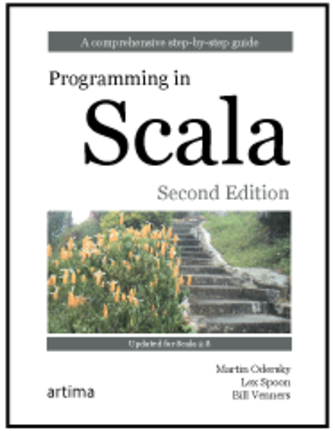
\includegraphics[height=0.4\textheight]{figs/programming-in-scala.pdf}
\end{center}

\end{columns}
\end{frame}

\begin{frame}[fragile]{Scala Functional}

\begin{scala}
def f (x: Int) = 2 * x

def g (xs: List[Int]) =  xs.map(f)
\end{scala}
\end{frame}

\begin{frame}[fragile]{Scala Object Oriented}

\begin{scala}
object Blimp {
  var numBlimps = 0
  def apply(r: Double) = {
    numBlimps += 1
    new Blimp(r)
  }
}

Blimp.numBlimps
Blimp(10.0)

class Blimp(r: Double) {
  val rad = r
  println("Another Blimp")
}

class Zep(r: Double) extends Blimp(r)
\end{scala}

\end{frame}

\begin{frame}[fragile]{Scala Collections}
\begin{scala}
// Array's
val tbl = new Array[Int](256)
tbl(0) = 32
val y = tbl(0)
val n = tbl.length

// ArrayBuffer's
val buf = new ArrayBuffer[Int]()
buf += 12
val z = buf(0)
val l = buf.length

// List's
val els = List(1, 2, 3)
val a :: b :: c :: Nil = els
val m = els.length
\end{scala}
\end{frame}

\begin{frame}[fragile]{Scala Iteration}
\begin{scala}
val tbl = new Array[Int](256)

// loop over all indices
for (i <- 0 until tbl.length)
  tbl(i) = i

// loop of each sequence element
for (e <- tbl)
  tbl(i) += e

// nested loop
for (i <- 0 until 16; j <- 0 until 16)
  tbl(j*16 + i) = i

// create second table with doubled elements
val tbl2 = for (i <- 0 until 16) yield tbl(i)*2
\end{scala}
\end{frame}

\begin{frame}[fragile]{Scala Console}
\begin{scala}
scala
1 + 2
def f (x: Int) = 2 * x
f(4)
\end{scala}
\end{frame}

\begin{frame}[fragile]
\frametitle{Algebraic Graph Construction}

\begin{columns}
\column{0.35\textwidth}
{\lstset{basicstyle={\Large\ttfamily}}
\begin{scala}
Mux(x > y, x, y)
\end{scala}
}

\column{0.6\textwidth}

\begin{center}
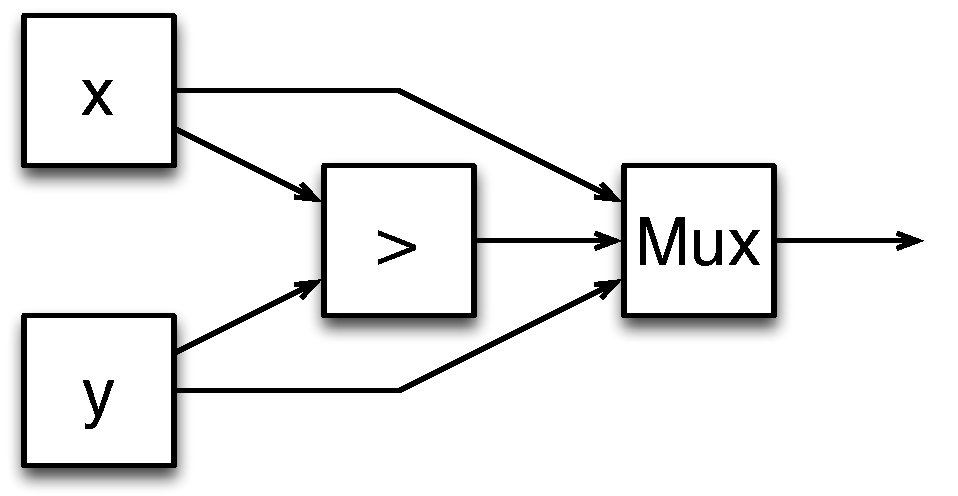
\includegraphics[width=0.9\textwidth]{figs/max2.pdf} 
\end{center}
\end{columns}
\end{frame}

\begin{frame}[fragile]
\frametitle{Creating Component}

\begin{columns}
\column{0.45\textwidth}

{\lstset{basicstyle={\scriptsize\ttfamily}}
\begin{scala}
class Max2 extends Component {
  val io = new Bundle {
    val x = UFix(width = 8).asInput
    val y = UFix(width = 8).asInput
    val z = UFix(width = 8).asOutput }
  io.z := Mux(io.x > io.y, io.x, io.y)
}
\end{scala}
}

\column{0.45\textwidth}
\begin{center}
\includegraphics[width=0.95\textwidth]{figs/Max2c.pdf} \\
\end{center}
\end{columns}

\end{frame}

\begin{frame}[fragile]
\frametitle{Connecting Components}

\begin{columns}
\column{0.25\textwidth}
\begin{scala}
val m1 = new Max2()
m1.io.x := a
m1.io.y := b
val m2 = new Max2()
m2.io.x := c
m2.io.y := d
val m3 = new Max2()
m3.io.x := m1.io.z
m3.io.y := m2.io.z
\end{scala}

\column{0.7\textwidth}

\begin{center}
\includegraphics[width=0.99\textwidth]{figs/Max4.pdf} \\
\end{center}
\end{columns}

\end{frame}


\begin{frame}[fragile]
\frametitle{Defining Construction Functions}

\begin{columns}

\column{0.45\textwidth}

\begin{scala}
def Max2 = Mux(x > y, x, y)
\end{scala}
\begin{scala}
Max2(x, y)
\end{scala}

\column{0.5\textwidth}

\begin{center}
\includegraphics[width=0.95\textwidth]{figs/Max2.pdf} \\[1cm]
\end{center}

\end{columns}

\end{frame}

\begin{frame}[fragile]
\frametitle{Functional Construction}

\begin{columns}

\column{0.45\textwidth}

\begin{scala}
Reduce(Array(a, b, c, d), Max2)
\end{scala}

\column{0.5\textwidth}

\begin{center}
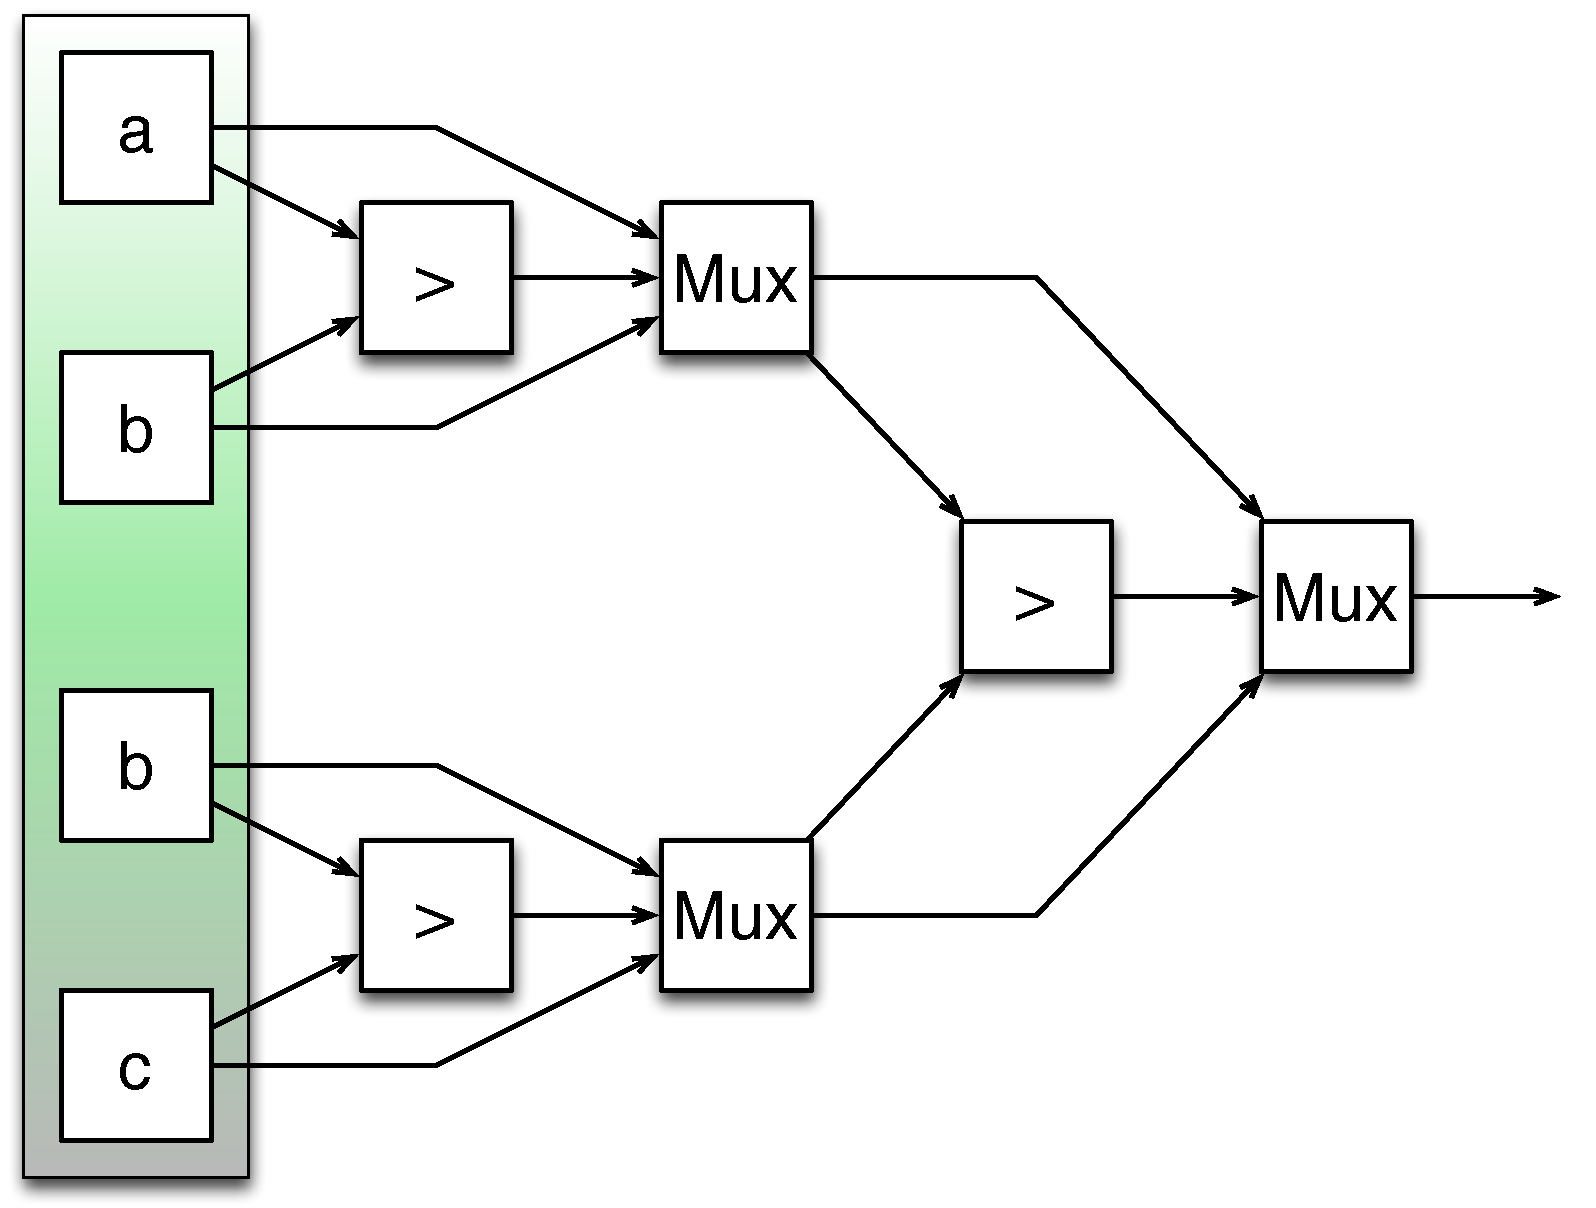
\includegraphics[width=0.99\textwidth]{figs/reduceMax.pdf} \\
\end{center}

\end{columns}

\end{frame}

\begin{frame}[fragile]
\frametitle{Example}
\begin{columns}

\column{0.45\textwidth}

\begin{footnotesize}
\begin{scala}
class GCD extends Component {
  val io = new Bundle {
    val a     = UFix(INPUT, 16)
    val b     = UFix(INPUT, 16)
    val z     = UFix(OUTPUT, 16)
    val valid = Bool(OUTPUT) }
  val x = Reg(resetVal = io.a)
  val y = Reg(resetVal = io.b)
  when (x > y) {
    x := x - y
  } .otherwise {
    y := y - x
  }
  io.z     := x
  io.valid := y === UFix(0)
}
\end{scala}
\end{footnotesize}

\column{0.45\textwidth}

\begin{center}
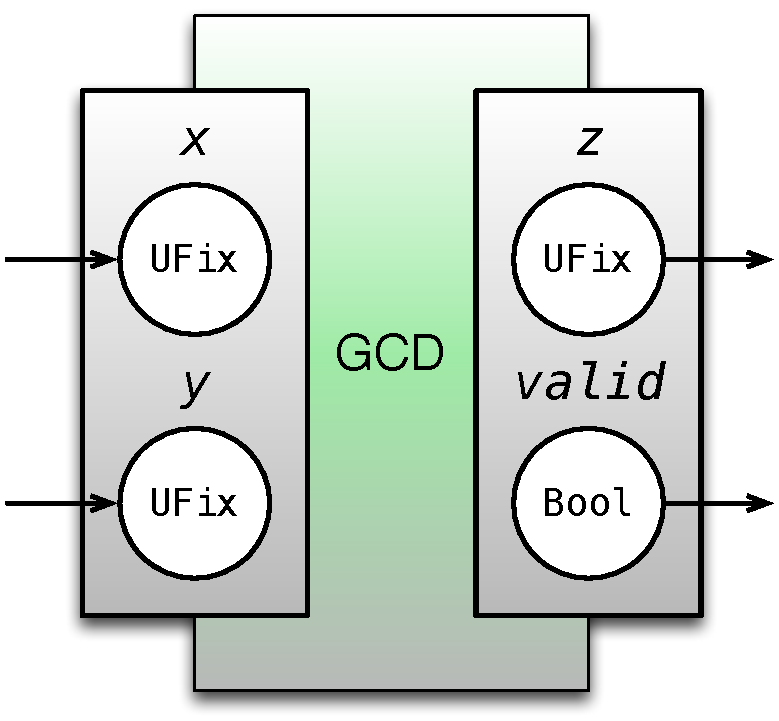
\includegraphics[width=0.9\textwidth]{figs/gcd.pdf} 
\end{center}

\end{columns}
\end{frame}

% \begin{frame}[fragile]{Scala Console}
% \begin{FramedVerb}
% \end{FramedVerb}
% \end{frame}

\begin{frame}[fragile]{Literals}
\begin{scala}
Bits(1)       // decimal 1-bit literal from Scala Int. 
Bits("ha")    // hexadecimal 4-bit literal from string.
Bits("o12")   // octal 4-bit literal from string. 
Bits("b1010") // binary 4-bit literal from string.

Fix(5)        // signed decimal 4-bit literal from Scala Int.
Fix(-8)       // negative decimal 4-bit literal from Scala Int.
UFix(5)       // unsigned decimal 3-bit literal from Scala Int.

Bool(true)    // Bool literals from Scala literals.
Bool(false)
\end{scala}
\end{frame}
 
\begin{frame}[fragile]{Literals}
\begin{scala}
Bits("h_dead_beef") // 32-bit literal of type Bits.
Bits(1)             // decimal 1-bit literal from Scala Int.
Bits("ha", 8)       // hexadecimal 8-bit literal of type Bits.
Bits("o12", 6)      // octal 6-bit literal of type Bits.
Bits("b1010", 12)   // binary 12-bit literal of type Bits.

Fix(5, 7)           // signed decimal 7-bit literal of type Fix.
UFix(5, 8)          // unsigned decimal 8-bit literal of type UFix.
\end{scala}
\end{frame}

\begin{frame}[fragile]{Type Hierarchy}

\begin{center}
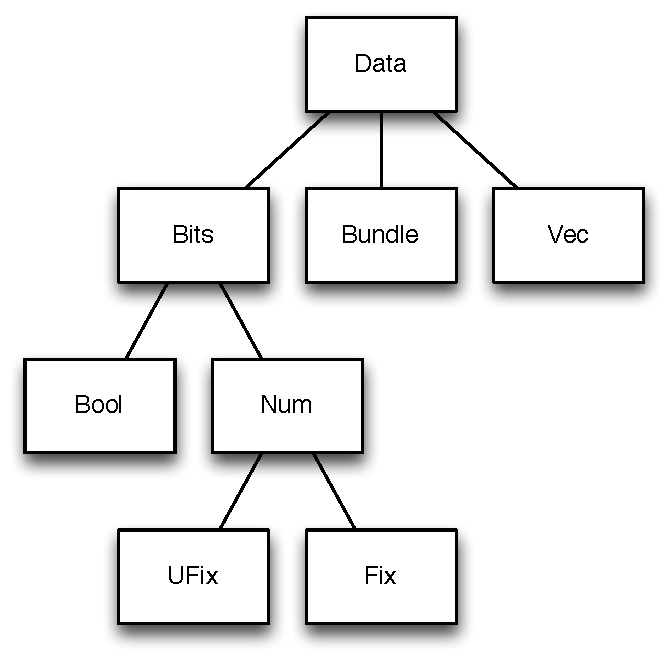
\includegraphics[height=0.9\textheight]{../manual/figs/type-hierarchy.pdf}
\end{center}

\end{frame}

\begin{frame}[fragile]{Combinational Circuits}
\begin{scala}
(a & b) | (~c & d)
\end{scala}
\begin{scala}
val sel = a | b
val out = (sel & in1) | (~sel & in0)
\end{scala}
\end{frame}

\begin{frame}[fragile]{Building Graphs}
\begin{center}
\begin{tabular}{ccc}
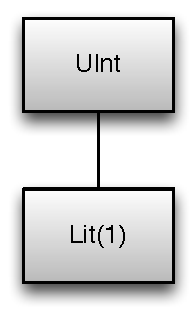
\includegraphics[height=0.94in]{../manual/figs/bits-1.pdf} &
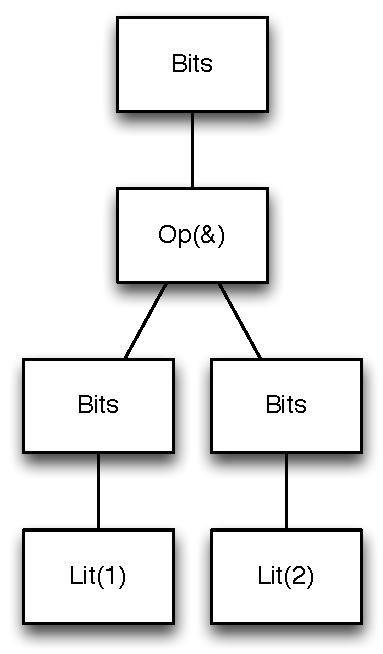
\includegraphics[height=1.96in]{../manual/figs/bits-and.pdf} &
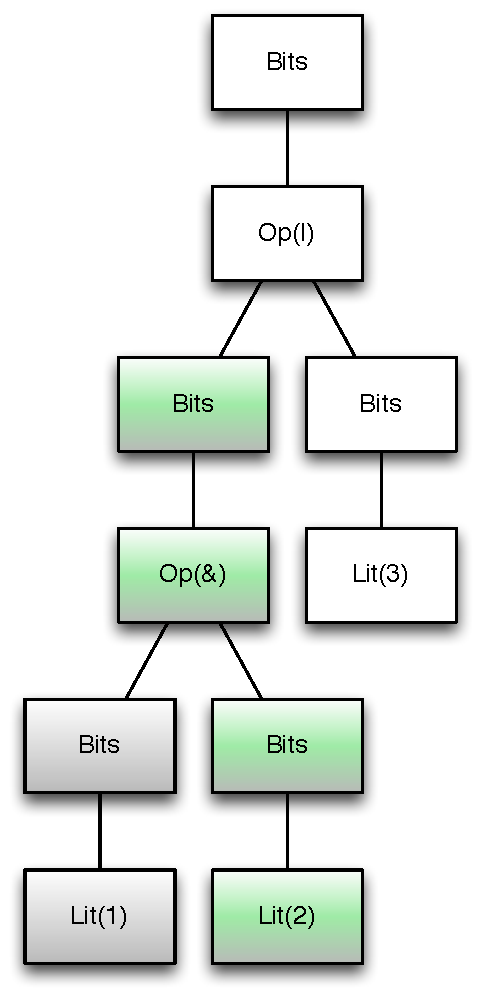
\includegraphics[height=3.0in]{../manual/figs/bits-or-and.pdf} \\
\code{a = Bits(1)} & \code{b = a \& Bits(2)} &
\code{b | Bits(3)} \\
\end{tabular}
\end{center}
\end{frame}

\begin{frame}[fragile]{Bitwise operators}
\textbf{Valid on Bits, Fix, UFix, Bool.}
\begin{scala}
// Bitwise-NOT
val invertedX = ~x                      
// Bitwise-AND 
val hiBits    = x & Bits("h_ffff_0000") 
// Bitwise-OR
val flagsOut  = flagsIn | overflow      
// Bitwise-XOR
val flagsOut  = flagsIn ^ toggle        
\end{scala}
\end{frame}

\begin{frame}[fragile]{Bitwise reductions}
\textbf{Valid on Bits, Fix, and UFix.  Returns Bool.}
\begin{scala}
// AND-reduction 
val allSet = andR(x)  
// OR-reduction
val anySet = orR(x)   
// XOR-reduction 
val parity = xorR(x)  
\end{scala}
\end{frame}

\begin{frame}[fragile]{Equality comparison}
\textbf{Valid on Bits, Fix, UFix, and Bool. Returns Bool.}
\begin{scala}
// Equality
val equ = x === y 
// Inequality 
val neq = x != y   
\end{scala}
\end{frame}

\begin{frame}[fragile]{Shifts}
\textbf{Valid on Bits, Fix, and UFix.}
\begin{scala}
// Logical left shift.
val twoToTheX = Fix(1) << x   
// Right shift (logical on Bits & UFix, arithmetic on Fix).
val hiBits    = x >> UFix(16) 
\end{scala}
\end{frame}

\begin{frame}[fragile]{Bitfield manipulation}
\textbf{Valid on Bits, Fix, UFix, and Bool.}
\begin{scala}
// Extract single bit, LSB has index 0.
val xLSB       = x(0)                
// Extract bit field  from end to start bit pos. 
val xTopNibble = x(15,12)            
// Replicate a bit string multiple times.
val usDebt     = Fill(3, Bits("hA")) 
// Concatenates bit fields, w/ first arg on left
val float      = Cat(sgn,exp,man)    
\end{scala}
\end{frame}

\begin{frame}[fragile]{Logical Operations}
\textbf{Valid on Bools. }
\begin{scala}
// Logical NOT. 
val sleep = !busy                     
// Logical AND.
val hit   = tagMatch && valid         
// Logical OR.
val stall = src1busy || src2busy      
// Two-input mux where sel is a Bool.  
val out   = Mux(sel, inTrue, inFalse) 
\end{scala}
\end{frame}

\begin{frame}[fragile]{Arithmetic operations}
\textbf{Valid on Nums: Fix and UFix. }
\begin{scala}
// Addition. 
val sum  = a + b  
// Subtraction.
val diff = a - b  
// Multiplication. 
val prod = a * b  
// Division.
val div  = a / b  
// Modulus
val mod  = a % b  
\end{scala}
\end{frame}

\begin{frame}[fragile]{Arithmetic comparisons}
\textbf{Valid on Nums: Fix and UFix. Returns Bool.}
\begin{scala}
// Greater than.
val gt  = a > b   
// Greater than or equal.
val gte = a >= b  
// Less than.
val lt  = a < b   
// Less than or equal.
val lte = a <= b  
\end{scala}
\end{frame}

\begin{frame}[fragile]{Bitwidth Inference}
\begin{center}
\begin{tabular}{ll}
{\bf operation} & {\bf bit width} \\ 
\verb|z = x + y| & \verb+wz = max(wx, wy)+ \\
\verb+z = x - y+ & \verb+wz = max(wx, wy)+\\
\verb+z = x & y+ & \verb+wz = max(wx, wy)+ \\
\verb+z = Mux(c, x, y)+ & \verb+wz = max(wx, wy)+ \\
\verb+z = w * y+ & \verb!wz = wx + wy! \\
\verb+z = x << n+ & \verb!wz = wx + maxNum(n)! \\
\verb+z = x >> n+ & \verb+wz = wx - minNum(n)+ \\
\verb+z = Cat(x, y)+ & \verb!wz = wx + wy! \\
\verb+z = Fill(n, x)+ & \verb+wz = wx * maxNum(n)+ \\
% \verb+z = x < y+ & \verb+<= > >= && || != ===+ & \verb+wz = 1+ \\
\end{tabular}
\end{center}
\end{frame}

\begin{frame}[fragile]{Node Class Hierarchy}

\begin{center}
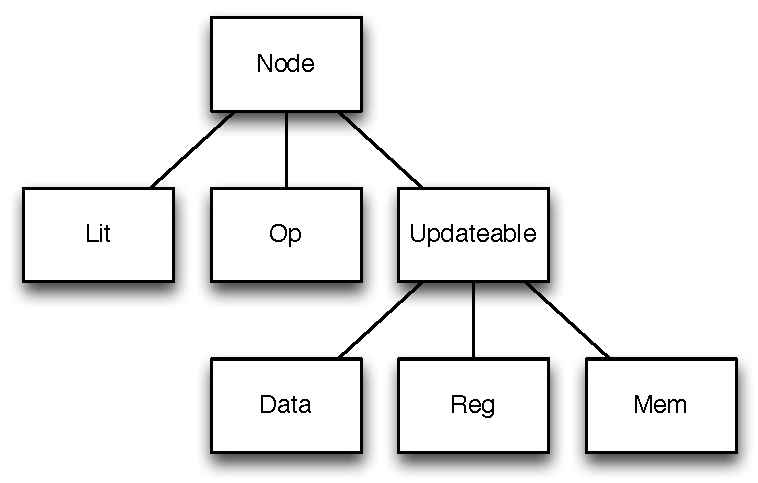
\includegraphics[height=0.9\textheight]{../manual/figs/node-hierarchy.pdf}
\end{center}

\end{frame}

\begin{frame}[fragile]{chisel repo}
\begin{FramedSemiVerb}
src                        \comment{\# chisel scala source code}
csrc                       \comment{\# chisel emulator source code}
doc                        \comment{\# documentation}
www                        \comment{\# web sources}
tutorial                   \comment{\# tutorial project}
tutorial/src               \comment{\# tutorial source code}
tutorial/sbt               \comment{\# tutorial sbt files}
tutorial/emulator          \comment{\# tutorial emulator build products}
tutorial/emulator/Makefile \comment{\# Makefile for emulator products} 
tutorial/verilog           \comment{\# tutorial verilog build products} 
tutorial/verilog/Makefile  \comment{\# Makefile for verilog products} 
\end{FramedSemiVerb}
\end{frame}

\begin{frame}[fragile]{Combinational -- \tt\small tutorial/src/combinational.scala}
\begin{scala}
package Tutorial

import Chisel._

class Combinational extends Component {
  val io = new Bundle {
    val x = UFix(INPUT, 16)
    val y = UFix(INPUT, 16)
    val z = UFix(OUTPUT, 16)
  }
  io.z := io.x + io.y
}
\end{scala}
\end{frame}

\begin{frame}[fragile]{Tutorial Main -- \tt tutorial/src/tutorial.scala}

\begin{scala}
package Tutorial

import Chisel._

object Tutorial {
  def main(args: Array[String]) = {
    val args = args.slice(1, args.length)
    args(0) match {
      case "combinational" => 
        chiselMain(args, () => new Combinational())
      ...
    }
  }
}
\end{scala}
\end{frame}


\setbeamercolor{frametitle}{bg=\frametitleproblemcolor}
\begin{frame}[fragile]{Emitting C++ and Compiling}

{\lstset{basicstyle={\tiny\ttfamily}}
\begin{scala}
def main(args: Array[String]) = {
 val args = args.slice(1, args.length)
  args(0) match {
    case "combinational" => chiselMain(args, () => new Combinational())
} }
\end{scala}

get into sbt directory:

\begin{scala}
cd $CHISEL/tutorial/sbt
\end{scala}

emit C++ and compile \code{tutorial/emulator/Combination-*} to
produce combinational circuit app named \code{tutorial/emulator/Combination}:

\begin{scala}
bash> sbt
sbt> project tutorial
sbt> compile
sbt> run Combinational --backend c --targetDir ../emulator --compile --genHarness
sbt> exit
\end{scala}

or on one line

\begin{scala}
sbt "project tutorial" "run Combinational --backend c --targetDir ../emulator --compile --genHarness"
\end{scala}
}
\end{frame}
\setbeamercolor{frametitle}{bg=\frametitledefaultcolor}

\begin{frame}{Chisel Workflow}
\begin{center}
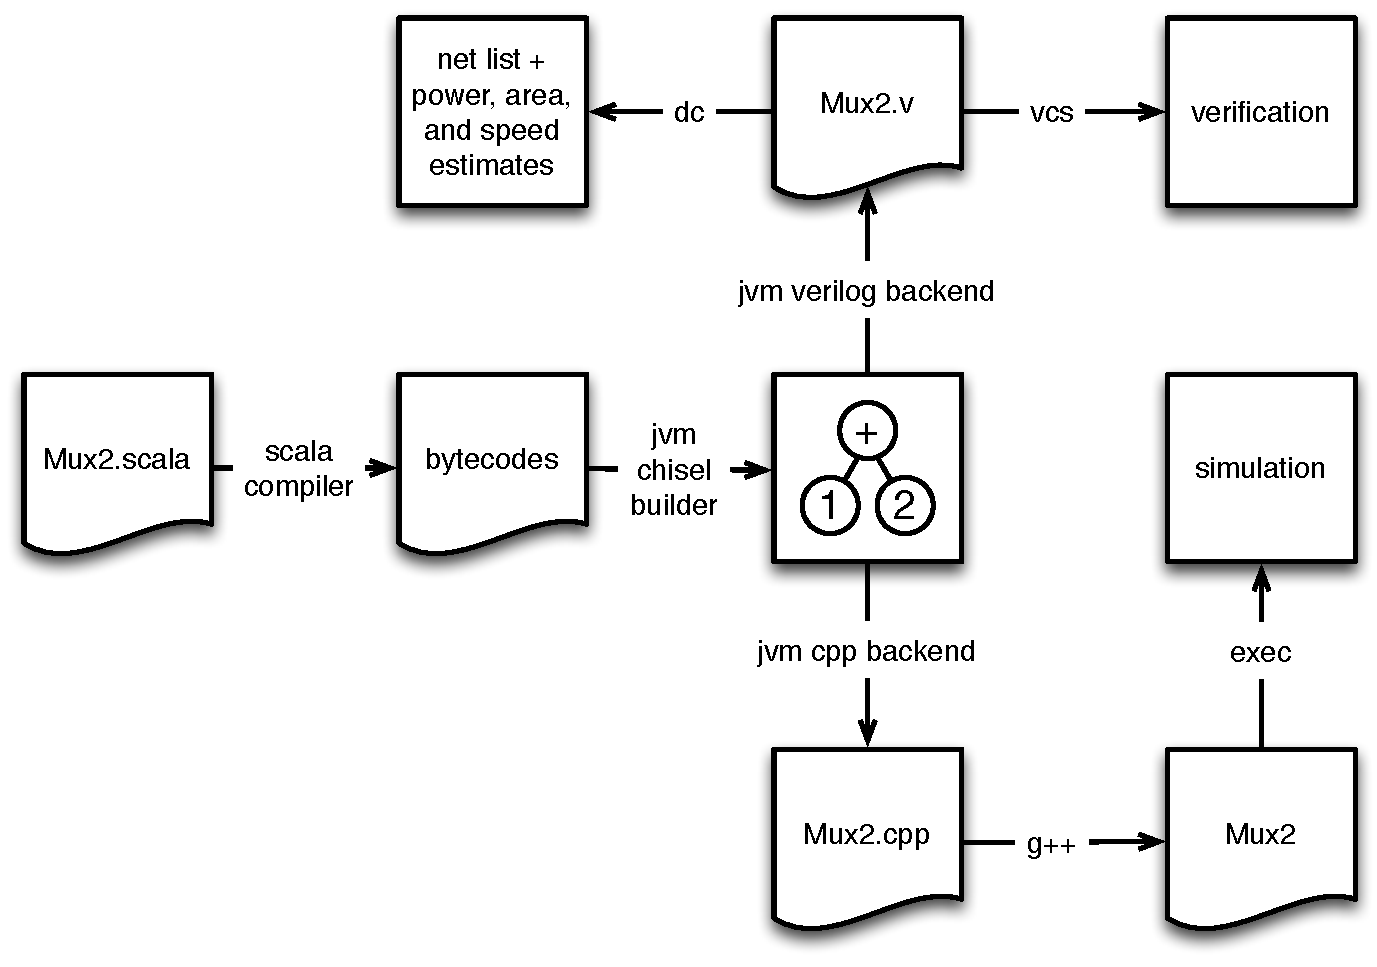
\includegraphics[height=0.9\textheight]{figs/chisel-workflow.pdf}
\end{center}
\end{frame}

\begin{frame}[fragile]{Defining a Tester}

\begin{columns}
\column{0.45\textwidth}
{\lstset{basicstyle={\tiny\ttfamily}}
\begin{scala}
package Tutorial
import Chisel._
import scala.collection.mutable.HashMap
import scala.util.Random

class Combinational extends Component {
  val io = new Bundle {
    val x = UFix(INPUT, 16)
    val y = UFix(INPUT, 16)
    val z = UFix(OUTPUT, 16) }
  io.z := io.x + io.y
}

class CombinationalTests(c: Combinational) 
    extends Tester(c, Array(c.io)) {
  defTests {
    var allGood = true
    val vars    = new HashMap[Node, Node]()
    val rnd     = new Random()
    val maxInt  = 1 << 16
    for (i <- 0 until 10) {
      vars.clear()
      val x        = rnd.nextInt(maxInt)
      val y        = rnd.nextInt(maxInt)
      vars(c.io.x) = UFix(x)
      vars(c.io.y) = UFix(y)
      vars(c.io.z) = UFix((x + y)&(maxInt-1))
      allGood      = step(vars) && allGood
    }
    allGood
} }
\end{scala}
}
\column{0.45\textwidth}
{\lstset{basicstyle={\tiny\ttfamily}}
\begin{scala}
class Tester[T <: Component]
  (val c: T, val testNodes: Array[Node])

def defTests(body: => Boolean)

def step(vars: HashMap[Node, Node]): Boolean
\end{scala}
}
\begin{tiny}
\begin{itemize}
\item user subclasses \code{Tester} defining DUT and
\code{testNodes} and tests in \code{defTests} body
\item \code{vars} is mapping from \code{testNodes} to literals, called bindings
\item \code{step} runs test with given bindings, where
var values for input ports are sent to DUT,
DUT computes next outputs, and
DUT sends next outputs to Chisel
\item finally \code{step} compares received values against var values
  for and returns false if any comparisons fail
  output ports
\end{itemize}
\end{tiny}

\begin{center}
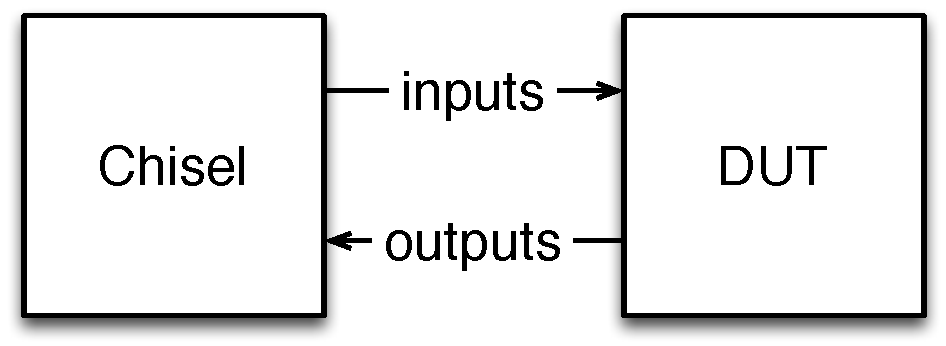
\includegraphics[width=0.9\textwidth]{figs/DUT.pdf}
\end{center}

\end{columns}
\end{frame}

\begin{frame}[fragile]{Binding Tester to Component}

\begin{scala}
object chiselMainTest {
  def apply[T <: Component]
    (args: Array[String], comp: () => T)(tester: T => Tester[T]): T
}
\end{scala}

\noindent and used as follows:

\begin{scala}
chiselMainTest(args + "--test", () => new Combinational()){ 
  c => new CombinationalTests(c) 
}
\end{scala}

\end{frame}

\setbeamercolor{frametitle}{bg=\frametitleproblemcolor}
\begin{frame}[fragile]{Running Tests Examples}

\begin{scala}
cd $CHISEL/tutorial/sbt
sbt "project tutorial" "run Combinational ... --compile --test"
...
PASSED
\end{scala}

or through makefile

\begin{scala}
cd $CHISEL/tutorial/emulator
make combinational
...
PASSED
\end{scala}

\end{frame}
\setbeamercolor{frametitle}{bg=\frametitledefaultcolor}

\begin{frame}[fragile]{Functional Abstraction}
\begin{scala}
def clb(a: Bits, b: Bits, c: Bits, d: Bits) = 
  (a & b) | (~c & d)

val out = clb(a,b,c,d)
\end{scala}
\end{frame}

\begin{frame}[fragile]{Functional Scala}
\begin{scala}
class Functional extends Component {
  def clb(a: Bits, b: Bits, c: Bits, d: Bits) = 
    (a & b) | (~c & d)
  val io = new Bundle {
    val x = Bits(INPUT, 16)
    val y = Bits(INPUT, 16)
    val z = Bits(OUTPUT, 16)
  }
  io.z := clb(io.x, io.y, io.x, io.y)
}
\end{scala}
\end{frame}

\begin{frame}[fragile]{Bundles}
\begin{scala}
class MyFloat extends Bundle {
  val sign        = Bool()
  val exponent    = UFix(width = 8)
  val significand = UFix(width = 23)
}

val x  = new MyFloat()
val xs = x.sign
\end{scala}
\end{frame}

\begin{frame}[fragile]{Vecs}
\begin{scala}
// Vector of 5 23-bit signed integers.
val myVec = Vec(5) { Fix(width = 23) } 

// Connect to one static element of vector.
val reg3  = myVec(3)                   
reg3     := data3 
myVec(4) := data4

// Connect to one dynamic element of vector.
val reg       = myVec(addr)
reg          := data1
myVec(addr2) := data2
\end{scala}
\end{frame}

\begin{frame}[fragile]{Ports}

\textbf{Data object with directions assigned to its members}

\begin{scala}
class FIFOInput extends Bundle {
  val ready = Bool(OUTPUT)
  val bits  = Bits(INPUT, 32)
  val valid = Bool(INPUT)
}
\end{scala}

\textbf{Direction assigned at instantiation time}

\begin{scala}
class ScaleIO extends Bundle {
  val in    = new MyFloat().asInput
  val scale = new MyFloat().asInput
  val out   = new MyFloat().asOutput
}
\end{scala}
\end{frame}

\begin{frame}[fragile]{Component}

\begin{itemize}
\item inherits from \verb+Component+,
\item contains an interface stored in a port field named \verb+io+, and
\item wires together subcircuits in its constructor.
\end{itemize}

\begin{scala}
class Mux2 extends Component {
  val io = new Bundle{
    val sel = Bits(INPUT, 1)
    val in0 = Bits(INPUT, 1)
    val in1 = Bits(INPUT, 1)
    val out = Bits(OUTPUT, 1)
  }
  io.out := (io.sel & io.in1) | (~io.sel & io.in0)
}
\end{scala}

\end{frame}

\begin{frame}[fragile]{chiselMain Command Line Arguments}
\begin{scala}
sbt 
sbt> project tutorial
sbt> compile                     // compiles Chisel Scala code
sbt> run Combinational           // produces C++ files
sbt> run Combinational --compile // produces C++ files and compiles
sbt> run Combinational --test    // produces C++ files, compiles, tests
sbt> exit
\end{scala}

with a complete set of command line arguments being:\\[2mm]

\begin{tabular}{lll}
\verb+--targetDir+ & target pathname prefix \\
\verb+--genHarness+ & generate harness file for C++ \\
\verb+--debug+ & put all wires in C++ class file \\
\verb+--compile+ & compiles generated C++ \\
\verb+--test+ & runs tests using C++ app \\
\verb+--backend v+ & generate verilog \\
\verb+--backend c+ & generate C++ (default)\\
\verb+--vcd+ & enable vcd dumping \\
\end{tabular}
\end{frame}

\begin{frame}[fragile]{Creating Verilog}

\begin{scala}
cd $CHISEL/tutorial/sbt; sbt "project tutorial" "run Mux2 --backend v ..."
\end{scala}

or through makefile:

\begin{scala}
cd $CHISEL/tutorial/verilog; make Mux2.v
\end{scala}

producing \code{Mux2.v}:

{\lstset{basicstyle={\tiny\ttfamily}}
\begin{scala}
module Mux2(
    input  io_sel,
    input  io_in0,
    input  io_in1,
    output io_out);

  wire T0;
  wire T1;
  wire T2;
  wire T3;

  assign io_out = T0;
  assign T0 = T3 | T1;
  assign T1 = T2 & io_in0;
  assign T2 = ~ io_sel;
  assign T3 = io_sel & io_in1;
endmodule
\end{scala}
}

\end{frame}

\begin{frame}[fragile]{Producing VCD}

\begin{scala}
cd $CHISEL/tutorial/sbt
sbt "project tutorial" "run Mux2 --backend c ... --vcd --compile --test"
\end{scala}

which then produces

\begin{scala}
$CHISEL/tutorial/emulator/Mux2.vcd
\end{scala}

which you can view with a vcd viewer
\end{frame}

\setbeamercolor{frametitle}{bg=\frametitleproblemcolor}
\begin{frame}[fragile]{Component Hierarchy Problem -- \tt Mux4.scala}
\begin{itemize}
\item child components stored in fields of parent
\item now write 4-to-1 mux out of 3 2-to-1 mux's
\end{itemize}
\begin{scala}
class Mux4 extends Component {
  val io = new Bundle {
    val in0 = Bits(INPUT, 1)
    val in1 = Bits(INPUT, 1)
    val in2 = Bits(INPUT, 1)
    val in3 = Bits(INPUT, 1)
    val sel = Bits(INPUT, 2)
    val out = Bits(OUTPUT, 1)
  }
  val m0 = new Mux2()
  m0.io.sel := io.sel(0); m0.io.in0 := io.in0; m0.io.in1 := io.in1

  // flush this out ...

  io.out := io.in0 & io.in1 & io.in2 & io.in3 & io.sel 
}
\end{scala}

\end{frame}
\setbeamercolor{frametitle}{bg=\frametitledefaultcolor}

\setbeamercolor{frametitle}{bg=\frametitleproblemcolor}
\begin{frame}[fragile]{Doing Mux4 Problem -- \tt Mux4.scala}
\begin{itemize}
\item loop
\begin{itemize}
\item edit and flush out Mux4.scala 
\item make Mux4
\end{itemize}
\item until PASSES
\end{itemize}
\begin{scala}
cd $CHISEL/tutorial/emulator
make Mux4
...
PASSED
\end{scala}
\end{frame}
\setbeamercolor{frametitle}{bg=\frametitledefaultcolor}

% \begin{frame}[fragile]{Running Examples By Hand}
% 
% \begin{scala}
% cd $CHISEL/tutorial/sbt 
% sbt "project tutorial" "run"
% cd ../emulator
% make -f Mux2-makefile
% \end{scala}
% 
% \end{frame}

\begin{frame}[fragile]{State Elements}

\begin{scala}
Reg(in)
\end{scala}

\begin{scala}
def risingEdge(x: Bool) = x && !Reg(x)
\end{scala}

\end{frame}

\begin{frame}[fragile]{Counter}

\begin{scala}
def wrapAround(n: UFix, max: UFix) =
  Mux(n > max, UFix(0), n)

def counter(max: UFix) = {
  val x = Reg(resetVal = UFix(0, max.getWidth))
  x := wrapAround(x + UFix(1), max)
  x
}
\end{scala}

\end{frame}

\begin{frame}[fragile]{Sequential Circuits}

\begin{scala}
// Produce pulse every n cycles.
def pulse(n: UFix) = counter(n - UFix(1)) === UFix(0)
\end{scala}

\begin{scala}
// Flip internal state when input true.
def toggle(p: Bool) = {
  val x = Reg(resetVal = Bool(false))
  x := Mux(p, !x, x)
  x
}
\end{scala}

\begin{scala}
// Square wave where each half cycle has given period.
def squareWave(period: UFix) = toggle(pulse(period))
\end{scala}

\end{frame}

\setbeamercolor{frametitle}{bg=\frametitleproblemcolor}
\begin{frame}[fragile]{Sequential Circuit Problem -- \tt Accumulator.scala}
\begin{itemize}
\item write sequential circuit that sums \code{in} values
\end{itemize}
\begin{scala}
class Accumulator extends Component {
  val io = new Bundle {
    val in  = UFix(INPUT, 1)
    val out = UFix(OUTPUT, 8)
  }

  // flush this out ...

  io.out := UFix(0)
}
\end{scala}
\end{frame}
\setbeamercolor{frametitle}{bg=\frametitledefaultcolor}

\begin{frame}[fragile]{Forward Declarations}

\begin{scala}
val pcPlus4      = UFix() 
val branchTarget = UFix()
val pcNext       = Mux(io.ctl.pcSel, branchTarget, pcPlus4)
val pcReg        = Reg(data = pcNext, resetVal = UFix(0, 32)) 
pcPlus4         := pcReg + UFix(4) 
... 
branchTarget    := addOut
\end{scala}

\end{frame}

\begin{frame}[fragile]{Conditional Updates}

\begin{scala}
val r = Reg() { UFix(16) }
when (c === UFix(0) ) {
  r := r + UFix(1)
}
\end{scala}

\end{frame}

\begin{frame}[fragile]{Conditional Updates Priority}

\begin{scala}
when (c1) { r := Bits(1) }
when (c2) { r := Bits(2) }
\end{scala}

\textbf{Conditional Update Order:}

\begin{center}
\begin{tabular}{|c|c|c|l|}
\hline
\code{c1} & \code{c2}  &  \code{r} & \\
\hline
0 &  0 & r &  \code{r} unchanged \\
0 &  1 & 2 & \\
1 &  0 & 1 & \\
1 &  1 & 2& \code{c2} takes precedence over \code{c1} \\
\hline
\end{tabular}
\end{center}

\end{frame}

\begin{frame}[fragile]{Conditional Update Synthesized Hardware}

\begin{center}
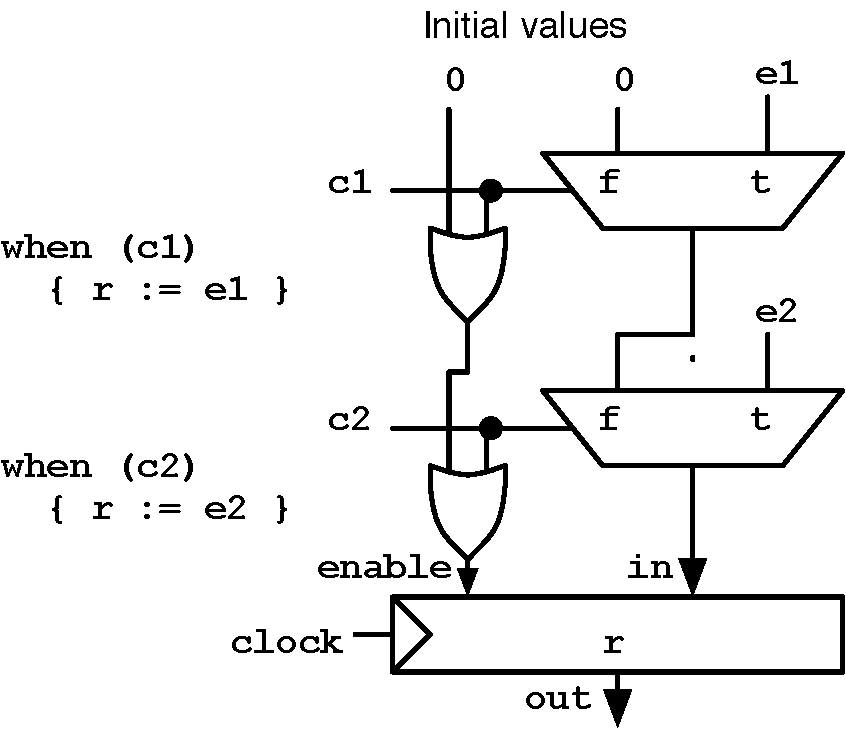
\includegraphics[height=2in]{figs/condupdates.pdf}
\end{center}

\begin{itemize}
\item Each \code{when} statement adds another level of data mux and ORs
  the predicate into the enable chain and
\item the compiler effectively adds
  the termination values to the end of the chain automatically.
\end{itemize}

\end{frame}

\begin{frame}[fragile]{Targetting Multiple Registers}

\begin{scala}
r := Fix(3) 
s := Fix(3)
when (c1) { r := Fix(1); s := Fix(1) }
when (c2) { r := Fix(2) }
\end{scala}

leads to \code{r} and \code{s} being updated according to the
following truth table:

{\footnotesize
\begin{center}
\begin{tabular}{|c|c|c|c|l|}
\hline
\code{c1} & \code{c2}  & \code{r} & \code{s} & \\
\hline 
0 &  0 & 3 & 3 & \\
0 &  1 & 2 & 3 & \\ 
1 &  0 & 1 & 1 & \code{r} updated in \code{c2} block, \code{s} updated using default \\
1 &  1 & 2 & 1 & \\
\hline
\end{tabular}
\end{center}
}


\end{frame}

\begin{frame}[fragile]{Conditional Update Nesting}

\begin{scala}
when (a) { when (b) { body } }
\end{scala}

which is the same as:

\begin{scala}
when (a && b) { body }
\end{scala}

\end{frame}

\begin{frame}[fragile]{Conditional Update Chaining}

\begin{scala}
when (c1) { u1 }
.elsewhen (c2) { u2 }
.otherwise { ud }
\end{scala}

which is the same as:

\begin{scala}
when (c1) { u1 }
when (!c1 && c2) { u2 }
when (!(c1 || c2)) { ud }
\end{scala}

\end{frame}

\begin{frame}[fragile]{Switch Statement}

\begin{scala}
switch(idx) {
 is(v1) { u1 }
 is(v2) { u2 }
}
\end{scala}

which is the same as:

\begin{scala}
when (idx === v1) { u1 }
when (idx === v2) { u2 }
\end{scala}

\end{frame}

\begin{frame}[fragile]{Finite State Machines}

\begin{scala}
class Parity extends Component {
  val io = new Bundle {
    val in  = Bool(INPUT)
    val out = Bool(OUTPUT) }
  val s_even :: s_odd :: Nil = Enum(2){ UFix() }
  val state  = Reg(resetVal = s_even)
  when (io.in) {
    when (state === s_even) { state := s_odd  }
    .otherwise              { state := s_even }
  }
  io.out := (state === s_odd)
}
\end{scala}
\end{frame}

\setbeamercolor{frametitle}{bg=\frametitleproblemcolor}
\begin{frame}[fragile]{FSM Problem -- \tt VendingMachine.scala}
\begin{itemize}
\item write vending machine which needs accepts 20 cents or more before raising valid high
\end{itemize}
\begin{scala}
class VendingMachine extends Component {
  val io = new Bundle {
    val nickel = Bool(INPUT)
    val dime   = Bool(INPUT)
    val valid  = Bool(OUTPUT) }
  val sIdle :: s5 :: s10 :: s15 :: sOk :: Nil = Enum(5){ UFix() }
  val state = Reg(resetVal = sIdle)

  // flush this out ...

  io.valid := (state === sOk)
}
\end{scala}
\end{frame}
\setbeamercolor{frametitle}{bg=\frametitledefaultcolor}

\begin{frame}[fragile]{ROM}

\begin{scala}
def Vec[T <: Data](elts: Seq[T])(data: => T): Vec[T]
def Vec[T <: Data](elts: T*)(data: => T): Vec[T]
\end{scala}

\begin{scala}
val i = Array(UFix(1), UFix(2), UFix(4), UFix(8))
val m = Vec(i){ UFix(width = 32) }
val r = m(counter(UFix(3)))
\end{scala}

% \begin{scala}
% def sinTable (amp: Double, n: Int) = {
%   val ts = Range(0, n, 1).map(i => (i*2*Pi)/(n.toDouble-1) - Pi) 
%   Vec(ts.map(t => Fix(round(amp * sin(t))))){ Fix(width = 32) }
% }
% 
% def sinWave (amp: Double, n: Int) = 
%   sinTable(amp, n)(counter(UFix(n))
% \end{scala}

\end{frame}

\setbeamercolor{frametitle}{bg=\frametitleproblemcolor}
\begin{frame}[fragile]{Mul Lookup Table Problem -- \tt Mul.scala}
\begin{itemize}
\item write 16x16 multiplication table using \code{Vec}
\end{itemize}
\begin{scala}
class Mul extends Component {
  val io = new Bundle {
    val x   = UFix(INPUT, 4)
    val y   = UFix(INPUT, 4)
    val z   = UFix(OUTPUT, 8)
  }
  val muls = new Array[UFix](256)

  // flush this out ...

  io.z := UFix(0)
}
\end{scala}

\end{frame}
\setbeamercolor{frametitle}{bg=\frametitledefaultcolor}

\begin{frame}[fragile]{Memories}

\begin{scala}
def object Mem {
  def apply[T <: Data](n: Int, resetVal: T = null)(type: => T): Mem
}

class Mem[T <: Data]
    (val n: Int, val resetVal: T, val inits: Seq[T], type: () => T) 
      extends Updateable {
  def apply(addr: UFix): T
}
\end{scala}

\end{frame}

\begin{frame}[fragile]{Register File}

\begin{scala}
val regs = Mem(32){ Bits(width = 32) }
when (wr_en) {
  regs(wr_addr) := wr_data
}
val idat = regs(iaddr)
val mdat = regs(maddr)
\end{scala}

\end{frame}

% \begin{frame}[fragile]{Realistic Register File}
% 
% \begin{scala}
% val regfile = Mem(64){ Bits(width = 32) }
% // w_mask = bit_mask
% when (wen) {
%   regfile(addr_in) := data_in1
% }
% val read_data = Reg(regfile(addr_in))
% \end{scala}
% 
% \end{frame}

\setbeamercolor{frametitle}{bg=\frametitleproblemcolor}
\begin{frame}[fragile]{Table Problem -- \tt Memo.scala}
\begin{itemize}
\item write read/write table using \code{Mem}
\end{itemize}
\begin{scala}
class Memo extends Component {
  val io = new Bundle {
    val isWr    = Bool(INPUT)
    val wrAddr  = UFix(INPUT, 8)
    val wrData  = UFix(INPUT, 8)
    val isRd    = Bool(INPUT)
    val rdAddr  = UFix(INPUT, 8)
    val rdData  = UFix(OUTPUT, 8)
  }
  val mem = Mem(256){ UFix(width = 8) }

  // flush this out ...

  io.rdData := UFix(0)
}
\end{scala}
\end{frame}
\setbeamercolor{frametitle}{bg=\frametitledefaultcolor}

% \begin{frame}[fragile]{Audio Recorder}
% 
% \begin{scala}
% def audioRecorder(n: Int, in: UFix, UFix, button: Bool) = { 
%   val addr = counter(UFix(n))
%   val ram  = Mem(n){ UFix(width = 16) }
%   when (button) {  
%     ram(addr) := in
%   }
%   ram(Mux(button, UFix(0), addr))
% } 
% \end{scala}
% 
% \end{frame}

\begin{frame}[fragile]{Port Classes, Subclasses, and Nesting}

\begin{scala}
class LinkIO extends Bundle { 
  val data  = Bits(16, OUTPUT) 
  val valid = Bool(OUTPUT)
}
\end{scala}

\noindent
We can then extend \verb+SimpleLink+ by adding parity bits using
bundle inheritance:

\begin{scala}
class PLinkIO extends LinkIO { 
  val parity = Bits(5, OUTPUT) 
}
\end{scala}

\noindent
In general, users can organize their interfaces into hierarchies using inheritance.  

\end{frame}

\begin{frame}[fragile]{Filter Example}

From there we can define a filter interface by nesting two
\verb+LinkIO+s into a new \verb+FilterIO+ bundle:

\begin{scala}
class FilterIO extends Bundle { 
  val in  = new LinkIO().flip
  val out = new LinkIO()
}
\end{scala}

\noindent
where \verb+flip+ recursively changes the ``gender'' of a bundle,
changing input to output and output to input.

We can now define a filter by defining a filter class extending component:

\begin{scala}
class Filter extends Component { 
  val io  = new FilterIO()
  io.out.valid := io.in.valid
  io.out.data  := io.in.data
}
\end{scala}

\noindent 
where the \verb+io+ field contains \verb+FilterIO+. 

\end{frame}

\setbeamercolor{frametitle}{bg=\frametitleproblemcolor}
\begin{frame}[fragile]{Even Filter Problem -- \tt Filter.scala}
\begin{itemize}
\item write filter that filters out even numbers
\end{itemize}
\begin{scala}
class Filter extends Component { 
  val io  = new FilterIO()

  // flush this out ...

  io.out.valid := Bool(true)
  io.out.data  := Bits(0)
}
\end{scala}
\end{frame}
\setbeamercolor{frametitle}{bg=\frametitledefaultcolor}

\begin{frame}[fragile]{Testing Decoupled Circuits}

\begin{scala}
class GCDTests(c: GCD) extends Tester(c, Array(c.io)) {
  defTests {
    val (a, b, z) = (64, 48, 16)
    val svars = new HashMap[Node, Node]()
    val ovars = new HashMap[Node, Node]()
    var t = 0
    do {
      svars(c.io.a) = UFix(a)
      svars(c.io.b) = UFix(b)
      step(svars, ovars)
      t += 1
    } while (t <= 1 || ovars(c.io.v).litValue() == 0)
    ovars(c.io.z).litValue() == z
  }
}
\end{scala}

\end{frame}

\begin{frame}[fragile]{Bundle Vectors}

\begin{scala}
class CrossbarIO extends Bundle {
  val in  = Vec(2){ new LinkIO() }
  val sel = UFix(INPUT, 2)
  val out = Vec(2){ new LinkIO() }
}
\end{scala}

\noindent
where \verb+Vec+ takes a size as the first argument and a block
returning a port as the second argument.
% and \code{clone} binds the construction argument \code{n} to cloning.

\end{frame}

\begin{frame}[fragile]{Bundle Vectors Cloning}

\begin{scala}
class CrossbarIO(n: Int) extends Bundle {
  val in  = Vec(n){ new LinkIO() }
  val sel = UFix(INPUT, log2Up(n))
  val out = Vec(n){ new LinkIO() }
  override def clone() = new CrossbarIO(n).asInstanceOf[this.type]
}
\end{scala}

\noindent
where \code{clone} definition fixes cloning, by incorporating the crossbar construction argument \code{n} in cloning.

\end{frame}

\begin{frame}[fragile]{Bulk Connections}
We can now compose two filters into a filter block as follows:

\begin{scala}
class Block extends Component { 
  val io = new FilterIO()
  val f1 = new Filter()
  val f2 = new Filter()

  f1.io.in  <> io.in
  f1.io.out <> f2.io.in
  f2.io.out <> io.out
}
\end{scala}

\noindent
where \verb+<>+ bulk connects interfaces.
\begin{itemize}
\item Bulk connections connect leaf ports of the same name to each other.
\item After all connections are made and the circuit is being elaborated,
Chisel warns users if ports have other than exactly one connection to them.
\end{itemize}

\end{frame}

\begin{frame}[fragile]{Parameterized Functions}
\begin{scala}
def Mux[T <: Bits](c: Bool, con: T, alt: T): T

Mux(c, UFix(10), UFix(11))
\end{scala}

\noindent
yields a \code{UFix} wire because the \code{con} and \code{alt}
arguments are each of type \code{UFix}.
\end{frame}

\begin{frame}[fragile]{Parameterized Signal Processing}

\begin{equation}
y[t] = \sum_j w_j * x_j[t-j]
\end{equation}

\begin{scala}
def innerProductFIR[T <: Num] (w: Seq[T], x: T) = {
  val delays = Range(0, w.length).map(i => w(i) * delay(x, i))
  delays.foldRight(_ + _)
}

def delay[T <: Bits](x: T, n: Int): T =
  if (n == 0) x else Reg(delay(x, n - 1))
\end{scala}

\end{frame}

\begin{frame}[fragile]{Parameterized Classes}
\begin{scala}
class FilterIO[T <: Data]()(data: => T) extends Bundle { 
  val in  = data.asInput.flip
  val out = data.asOutput
}

class Filter[T <: Data]()(data: => T) extends Component { 
  val io = new FilterIO(){ data }
  ...
}
\end{scala}
\end{frame}

\begin{frame}[fragile]{Parameterized Classes Continued}
\begin{scala}
class FIFOIO[T <: Data]()(data: => T) extends Bundle {
  val ready = Bool(INPUT)
  val valid = Bool(OUTPUT)
  val bits  = data.asOutput
}

class PipeIO[+T <: Data]()(data: => T) extends Bundle {
  val valid = Bool(OUTPUT)
  val bits  = data.asOutput
}
\end{scala}
\end{frame}

\setbeamercolor{frametitle}{bg=\frametitleproblemcolor}
\begin{frame}[fragile]{Decoupled GCD Problem -- \tt RealGCD.scala}

\begin{scala}
class RealGCDInput extends Bundle {
  val a = Bits(width = 16)
  val b = Bits(width = 16)
}

class RealGCD extends Component {
  val io  = new Bundle {
    val in  = new FIFOIO(){ new RealGCDInput() }.flip()
    val out = new PipeIO(){ Bits(width = 16) }
  }

  // flush this out ...
}
\end{scala}

\end{frame}
\setbeamercolor{frametitle}{bg=\frametitledefaultcolor}


\begin{frame}[fragile]{Object Oriented FIFOIO}

{\lstset{basicstyle={\scriptsize\ttfamily}}
\begin{scala}
class EnqIO[T <: Data]()(data: => T) extends FIFOIO()(data) {
  def enq(dat: T): T = { valid := Bool(true); data := dat; dat }
  valid := Bool(false);
  for (io <- data.flatten.map(x => x._2))
    io := UFix(0, io.getWidth());
}

class DeqIO[T <: Data]()(data: => T) extends FIFOIO()(data) {
  flip()
  ready := Bool(false);
  def deq(b: Boolean = false): T = { ready := Bool(true); data }
}

class Filter[T <: Data]()(data: => T) extends Component {
  val io = new Bundle {
    val in  = new DeqIO(){ data }
    val out = new EnqIO(){ data }
  }
  when (io.in.valid && io.out.ready) {
    io.out.enq(io.in.deq())
  }
}
\end{scala}
}

\end{frame}

\begin{frame}[fragile]{Router Interface}

{\lstset{basicstyle={\scriptsize\ttfamily}}
\begin{scala}
class ReadCmd extends Bundle {
  val addr = UFix(width = 32)
}

class WriteCmd extends ReadCmd {
  val data = UFix(width = 32)
}

class Packet extends Bundle {
  val header = UFix(width = 8)
  val body   = Bits(width = 64)
}

class RouterIO(n: Int) extends Bundle {
  override def clone = new RouterIO(n).asInstanceOf[this.type]
  val reads   = new DeqIO(){ new ReadCmd() }
  val replies = new EnqIO(){ UFix(width = 8) }
  val writes  = new DeqIO(){ new WriteCmd() }
  val in      = new DeqIO(){ new Packet() }
  val outs    = Vec(n){ new EnqIO(){ new Packet() } }
}
\end{scala}
}

\end{frame}

\setbeamercolor{frametitle}{bg=\frametitleproblemcolor}
\begin{frame}[fragile]{Router Problem -- \tt Router.scala}
\begin{scala}
class Router extends Component {
  val depth = 32;
  val n     = 4;
  val io    = new RouterIO(n);
  val tbl   = Mem(depth){ UFix(width = sizeof(n)) };
  
  // flush it out ...
}
\end{scala}
\begin{center}
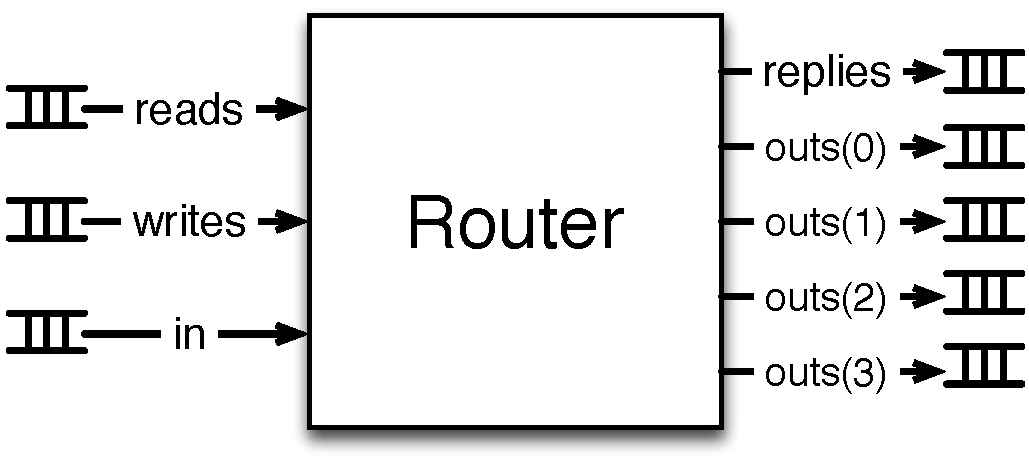
\includegraphics[height=0.45\textheight]{figs/trouter.pdf} 
\end{center}
\end{frame}
\setbeamercolor{frametitle}{bg=\frametitledefaultcolor}

\begin{frame}[fragile]{Advanced Topics}

\begin{itemize}
\item git
\item sbt
\item project directory structure
\item project file
\item installation
\end{itemize}

\end{frame}

\begin{frame}[fragile]{git}
\begin{FramedVerb}
cd ${HOME}
git clone git@github.com:ucb-bar/chisel.git
export CHISEL=${HOME}/chisel
git pull
git status 
git log
git add filename
git commit -m "comment"
git push
\end{FramedVerb}
\end{frame}

\begin{frame}[fragile]{sbt}
\begin{FramedVerb}
cd ${CHISEL}/tutorial/sbt
sbt
project tutorial
compile
run
console
\end{FramedVerb}
\end{frame}

\begin{frame}[fragile]{Project Directory Structure}
% \begin{footnotesize}
\begin{FramedSemiVerb}
chisel/
  tutorial/
  src/
gpu/
  sbt/
    project/build.scala \comment{\# edit this as shown below}
  src/                  \comment{\# your source files go here}
    gpu.scala           
  emulator/             \comment{\# your C++ target can go here}
\end{FramedSemiVerb}
% \end{footnotesize}

\end{frame}

\begin{frame}[fragile]{Project File}

{\lstset{basicstyle={\tiny\ttfamily}}
\begin{scala}
import sbt._
import Keys._

object BuildSettings {
  val buildOrganization = "edu.berkeley.cs"
  val buildVersion = "1.1"
  val buildScalaVersion = "2.9.2"

  def apply(projectdir: String) = {
    Defaults.defaultSettings ++ Seq (
      organization := buildOrganization,
      version      := buildVersion,
      scalaVersion := buildScalaVersion,
      scalaSource in Compile := Path.absolute(file(projectdir + "/src"))
    )
  }
}

object ChiselBuild extends Build {
  import BuildSettings._
  val chiselDir = System.getProperty(``CHISEL'')
  lazy val chisel = 
    Project("chisel", file("chisel"), 
            settings = BuildSettings(chiselDir))
  lazy val gpu =
    Project("gpu", file("gpu"), 
            settings = BuildSettings("..")) 
      dependsOn(chisel)
}
\end{scala}
}

\end{frame}

\begin{frame}[fragile]{Installation}
\begin{itemize}
\item on mac install:
\begin{itemize}
\item XCODE console tools
\item http://www.macports.org
\end{itemize}
\item on windows install:
\begin{itemize}
\item cygwin
\end{itemize}
\item everywhere install:
\begin{itemize}
\item git
\item g++
\item java
\end{itemize}
\item everywhere
\begin{itemize}
\item export \$CHISEL=...
\item git clone https://github.com/ucb-bar/chisel.git
\end{itemize}
\end{itemize}

\end{frame}

\begin{frame}[fragile]{Projects Ideas}

\begin{center}
\begin{tabular}{rl}
\textbf{audio processing} & \code{Echo.scala} \\
\textbf{image processing} & \code{Darken.scala} \\
\textbf{risc processor} & \code{Risc.scala} \\
\textbf{game of life} & \code{Life.scala} \\
\textbf{router} & \code{Router.scala} \\
\textbf{map/reduce} & \textit{see next slide}\\
\textbf{network} & \\
\textbf{fft} & \\
\textbf{cryptography} & \\
\textbf{serial multiplier} & \\
\textbf{pong} & \\
\end{tabular}
\end{center}

\end{frame}

\begin{frame}[fragile]{Functional Composition}
\begin{columns}

\column{0.45\textwidth}
\verb+Map(ins, x => x * y)+ \\
\begin{center}
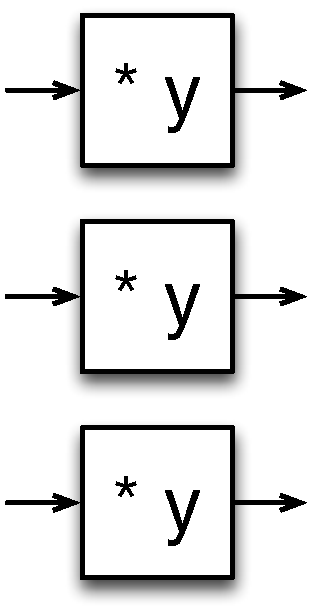
\includegraphics[height=0.6\textheight]{figs/map.pdf} \\[2cm]
\end{center}

\column{0.45\textwidth}
\vskip2mm
\verb+Chain(n, in, x => f(x))+ \\
\begin{center}
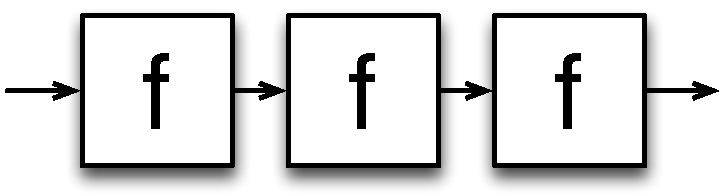
\includegraphics[width=0.9\textwidth]{figs/chain.pdf} \\
\end{center}

\verb+Reduce(data, Max)+ \\
\begin{center}
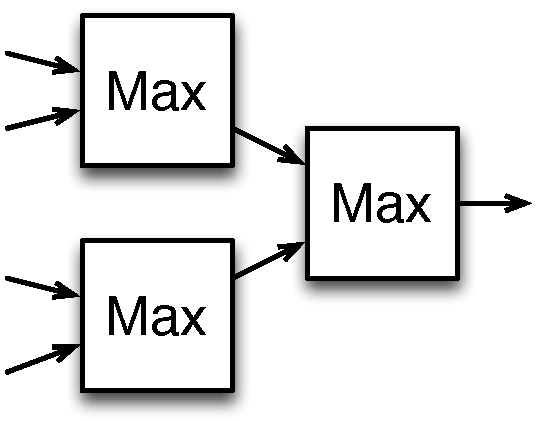
\includegraphics[width=0.9\textwidth]{figs/reduce.pdf} \\
\end{center}


\end{columns}
\end{frame}

\begin{frame}[fragile]{Keep in Touch}
\begin{center}
\begin{tabular}{rl}
\textbf{website} & \url{chisel.eecs.berkeley.edu} \\
\textbf{mailing list} & \url{groups.google.com/group/chisel-users} \\
\textbf{github} & \url{https://github.com/ucb-bar/chisel/} \\
\textbf{me} & \url{jrb@pobox.com} \\
\end{tabular}
\end{center}
\end{frame}

\begin{frame}{Thanks}
\begin{itemize}
\item \textbf{Arrangements} -- Roxana and Tammy
\item \textbf{EC2 configuration} -- Henry Cook and Michael Armbrust 
\item \textbf{Bootcamp Materials} -- Huy Vo and Andrew Waterman
\item \textbf{Dry Runs} -- Danny, Quan, and Albert
\item \textbf{Funding} -- Department of Energy
\end{itemize}
\end{frame}

% \begin{frame}[fragile]{Port Views}
% 
% {\lstset{basicstyle={\tiny\ttfamily}}
% \begin{scala}
% class RomIo extends Bundle {
%   val isVal = Bool(INPUT)
%   val raddr = UFix(INPUT, 32)
%   val rdata = Bits(OUTPUT, 32)
% }
% 
% class CpathIo extends Bundle() {
%   val imem = RomIo().flip()
%   val dmem = RamIo().flip()
%   ...
% }
% 
% class Cpu extends Component {
%   val io = new CpuIo()
%   val c  = new CtlPath()
%   val d  = new DatPath()
%   c.io.ctl  <> d.io.ctl
%   c.io.dat  <> d.io.dat
%   c.io.imem <> io.imem
%   d.io.imem <> io.imem
%   c.io.dmem <> io.dmem
%   d.io.dmem <> io.dmem
%   d.io.host <> io.host
% }
% \end{scala}
% }
% 
% \end{frame}
% 
% \begin{frame}[fragile, shrink]{Testing Examples}
% 
% \begin{scala}
% object tutorial {
%   def main(args: Array[String]) = {
%     chiselMainDebug(args ++ Array("--genHarness"), 
%                    () => new Mux2())(
%       c => Scanner("%x %x %x", c.io.sel, c.io.in0, c.io.in1),
%       c => Printer("%x %x %x %x", c.io.sel, c.io.in0, c.io.in1, c.io.out))
%   }
% }
% \end{scala}
% 
% compile
% 
% \begin{scala}
% sbt> run
% sbt> exit
% cd ../emulator
% make -f Mux2-makefile
% \end{scala}
% 
% \end{frame}
% 
% \begin{frame}[fragile, shrink]{Testing Examples Continued}
% 
% test.out
% 
% \begin{scala}
% 0 0 0 0
% 0 0 1 0
% 0 1 0 1
% 0 1 1 1
% 1 0 0 0
% 1 0 1 1
% 1 1 0 0
% 1 1 1 1
% \end{scala}
% 
% testing
% 
% \begin{scala}
% cut -f 1,2,3 -d " " < test | Mux2 > test.out
% diff test.out test
% \end{scala}
% 
% \end{frame}

\end{document}
